\documentclass[12pt]{article}
\usepackage{graphicx}
\usepackage{mathtools}
\topmargin -0.5in
\oddsidemargin -0.0in
\evensidemargin -0.0in
\textheight 9in
\textwidth 6.5in
\usepackage{hyperref}

\usepackage{mathptmx}
\usepackage{helvet}  
\usepackage{amsmath}
\usepackage{courier}    
\usepackage{type1cm}
\usepackage[noend,noline,boxed]{algorithm2e}
\usepackage{makeidx}    
\usepackage{graphicx}
\usepackage{subcaption}
\captionsetup{compatibility=false}
\usepackage{multicol} 
\usepackage{booktabs}
\usepackage{cite}
\usepackage[bottom]{footmisc}
\usepackage{xspace}
\usepackage[textsize=scriptsize,disable]{todonotes}
\usepackage{comment}

\usepackage{etex}

\usepackage{amsmath} % assumes amsmath package installed
\usepackage{amssymb}  % assumes amsmath package installed
\usepackage{amsfonts,amssymb}

%%%%%%
\usepackage[font=small]{caption}
\usepackage{units}
\usepackage{array}
\usepackage{tabulary}
\usepackage{verbatim}
\usepackage{booktabs}
\usepackage{multirow}
\usepackage{balance}
\usepackage{amsmath,amsfonts,amssymb} % this is handy for mathematicians and physicists
\usepackage[utf8]{inputenc}
%\usepackage[inline]{asymptote}
\usepackage{setspace}
\usepackage[noend,noline,boxed]{algorithm2e}
\usepackage{tabularx}
%\usepackage{algorithm}
\usepackage{algpseudocode}

\begin{document}
%\pagestyle{empty}

\title{Zenuity Sensor Fusion Task :  Object Tracking}
\author{Jay Patravali}


\maketitle \textbf{Problem Summary}

The problem is of tracking a submarine vessel using sonar sensor mounted on a boat. The sonar sensor records noisy measurements with standard deviation $\approx$  0.1
m in range, standard deviation  $\approx$ 3 degrees in angle. The vehicle initial belief state is taken as x and y equal to first groundtruth reading and zero x and y velocities.
Submarine has a constant velocity motion model.

\section{EKF Equations and Matrices}
Problem can be addressed using an Extended Kalman Filter. Equations for EFK are.

Model,
\begin{eqnarray}
x_k = f(x_{k-1})  + v_k \\
z_k = h_{k}(x_{k})  + w_k 
\end{eqnarray}

Predict,
\begin{eqnarray}
\hat{x}_k = Fx_{k-1} \\
P_k = F_{k} P_{k-1} F^T_{k} + Q_{k} 
\end{eqnarray}

Update,
\begin{eqnarray}
K = P_k H_k^T (H_k P_k H_k^T + R)^{-1} \\
\hat{x}_k = \hat{x}_{k} + K(z_{k} - h_{k}(\hat{x}_{k})) \\
P_k  = (I - K H_k) P_k
\end{eqnarray}

where matrices expand as ,

\[
x_{k-1}=
  \begin{bmatrix}
    x\\
    y\\
    vx\\
    vy
  \end{bmatrix}
\]


\[
F_{k}=
  \begin{bmatrix}
1 & 0 & Ts & 0\\
0 & 1  & 0 & Ts\\
0 & 0 & 1 &0\\
0 & 0 & 0 &1
  \end{bmatrix}
\]



\[
P_{k-1}=
  \begin{bmatrix}
1 & 0 & 0 & 0\\
0 & 1  & 0 & 0\\
0 & 0 & 1 &0\\
0 & 0 & 0 &1
  \end{bmatrix}
\]


\[
Q_{k} = q 		
  \begin{bmatrix}
Ts^{3}/3 & 0 & Ts^{2}/2 & 0\\
0 & Ts^{3}/3  & 0 & Ts^{2}/2\\
Ts^{2}/2 & 0 & Ts &0\\
0 & Ts^{2}/2 & 0 &Ts
  \end{bmatrix}
\]




\[
I =
  \begin{bmatrix}
1 & 0 & 0 & 0\\
0 & 1  & 0 & 0\\
0 & 0 & 1 &0\\
0 & 0 & 0 &1
  \end{bmatrix}
\]


\[
h_{k}(\hat{x}_{k})=
  \begin{bmatrix}
    r = \sqrt{  \hat{x}_k^{2} + \hat{y}_k^{2} } \\
    angle = tan^{-1} \frac{\hat{y}_k^{2}}{\hat{x}_k^{2}}\\

  \end{bmatrix}
\]

\[
z_{k}=
  \begin{bmatrix}
     meas\_range  \\
     meas\_angle\\

  \end{bmatrix}
\]


\[
H_{k} = \frac{\partial h}{\partial (x, y, vx, vy)} =
\begin{bmatrix}
\frac{\partial h}{\partial x} \sqrt{  \hat{x}_k^{2} + \hat{y}_k^{2}} & 0 & \frac{\partial h}{\partial y} \sqrt{  \hat{x}_k^{2} + \hat{y}_k^{2}} & 0\\
\frac{\partial h}{\partial x}tan^{-1} \frac{\hat{y}_k^{2}}{\hat{x}_k^{2}}  & 0 & \frac{\partial h}{\partial y}tan^{-1} \frac{\hat{y}_k^{2}}{\hat{x}_k^{2}} & 0\\

\end{bmatrix}
=
  \begin{bmatrix}
\frac{\hat{x_{k}}}{ \sqrt{\hat{x}_k^{2} + \hat{y}_k^{2}}} & \frac{\hat{y_{k}}}{ \sqrt{\hat{x}_k^{2} + \hat{y}_k^{2}}} & 0 & 0\\
\frac{-\hat{y_{k}}}{  \hat{x}_k^{2} + \hat{y}_k^{2}} & \frac{\hat{x}_k}{  \hat{x}_k^{2} + \hat{y}_k^{2}}  & 0 & 0\\

  \end{bmatrix}
\]

\begin{comment}

\[
h_{k}(\hat{x}_{k})=
  \begin{bmatrix}
     \hat{x}_k + n_{1}  \\
    \hat{y}_k + n_{2}\\

  \end{bmatrix}
\]


\[
z_{k}(\hat{x}_{k})=
  \begin{bmatrix}
     meas\_range * cos(meas\_angle)  \\
     meas\_range * sin(meas\_angle)\\

  \end{bmatrix}
\]


\[
H_{k} = \frac{\partial h}{\partial (x, y, vx, vy)} =
\begin{bmatrix}
\frac{\partial h}{\partial x} \hat{x}_k &   \frac{\partial h}{\partial x} \hat{y}_k & 0 & 0\\
\frac{\partial h}{\partial y} \hat{x}_k   &  \frac{\partial h}{\partial y} \hat{y}_k &  0 & 0\\

\end{bmatrix}
=
  \begin{bmatrix}
1 & 0 & 0 & 0\\
0 & 1 & 0 & 0\\
  \end{bmatrix}
\]
\end{comment}



\[
R =
  \begin{bmatrix}
\sigma_r^{2}  & 0\\
0 & \sigma_a^{2} \\
  \end{bmatrix}
\]

and these variables are described as follows ,
\begin{itemize}
    \item[$-$] $v_{k}$ is zero-mean gaussian process noise and $w_{k}$ is measurement noise of zero-mean gaussian distribution. 
    \item[$-$] $vx$ and $vy$ is velocities in $x$ and $y$ coordinates
    \item[$-$] $P_{k}$ is covariance of state, and $P_{k-1}$ is initial covariance
    \item[$-$] $F_{k}$ is state transition matrix
    \item[$-$] $Q_{k}$ is covariance matrix of process noise, $q$ is a tunable scaling factor.
	\item[$-$] $R$ is measurement noise covariance matrix, with $\sigma_{r}^{2}$ and $\sigma_{a}^{2}$ as variance in range and angle for a zero mean gaussian distribution.
    \item[$-$] $z_{k}$ is the observed measurements obtained from the sensor. In this case range and azimuth angle.
 
    \item[$-$] $h_{k}(\hat{x}_{k})$ is observation function that describes  measurements  predicted from the state in X and Y.
    \item[$-$] $H_{k}$ is jacobian of observation function $h_{k}(\hat{x}_{k})$ evaluated at the current estimate of the state from the prediction step.
    \item[$-$] $\hat{x}_{k}$ is mean  of distribution of state estimated by the EKF.
    \item[$-$] $K$ is the Kalman gain.


\begin{comment}
    \item[$-$] $z_{k}$ is the observed state derived from the measurements obtained from the sensor. In this case range and azimuth angle is transformed into X and Y states.
 
    \item[$-$] $h_{k}(\hat{x}_{k})$ is observation function that describes predicted state in X and Y with added gaussian noise -- $n_{1}$, $n_{2}$ that are drawn from $N(0, \sigma_{r}^{2})$ and $N(0, \sigma_{a}^{2})$ respectively. 
    \item[$-$] $H_{k}$ is jacobian of observation function $h_{k}(\hat{x}_{k})$ evaluated at the current estimate of the state from the prediction step.
    \item[$-$] $\hat{x}_{k}$ is mean  of distribution of state estimated by the EKF.
    \item[$-$] $K$ is the Kalman gain.
\end{comment}

\end{itemize}
\section{Generating sensor measurements}

Given the ground truth trajectory, we can assume the boat to be stationary at the origin, and calculate range and angle from this frame of reference.  We generate 100 such unique sequences each containing 500 measurements for corresponding ground truth value. The code and visualization is given in $scripts/generate_measurement.py$.

\begin{eqnarray}
\left.\begin{aligned}
range\_val & = vals\_x^{2} + vals\_y^{2}\\
noisy\_r & = range\_val + normal\_distribution(0, \sigma_{r})\\
azimuth & = math.atan(vals\_y/vals\_x)\\
noisy\_a & = azimuth + normal\_distribution(0, \sigma_{a})\\
\end{aligned}\right.
\end{eqnarray}

Where,  normal\_distribution()  is added zero-mean gaussian noise.  $vals\_x$ and $vals\_y$ is x and y coordinates from ground truth data. Here, $noisy_r$ is range with added zero-mean gaussian noise with std dev 0.1m
$noisy_a$ is range with added zero-mean gaussian noise with std dev $3*PI/180$ radians.
A single sequence is illustrated in Fig. \ref{fig:noisy_path_sample}.
\\
       
To run the code, just type  \texttt{python generate\_measurements.py} !

\begin{figure}[!h]
\centering
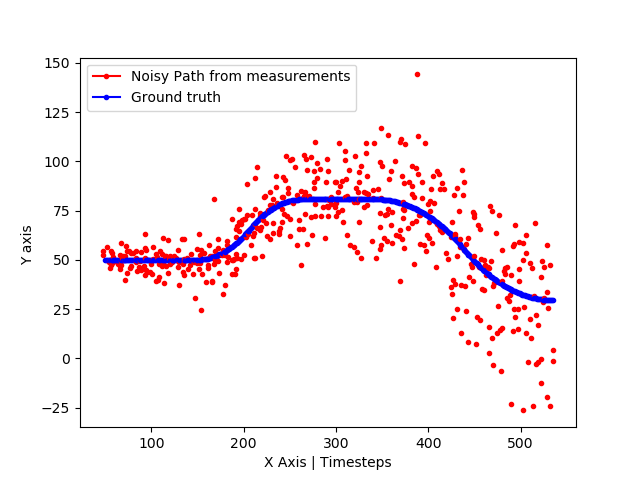
\includegraphics[width =4.0in]{../results/noisy_path_sample.png}
\caption{Path reconstructed from generated noisy measurements}
\label{fig:noisy_path_sample}
\end{figure}

       
\section{Running the  EFK and Results}
Code is setup to run for 100 EFK samples and plot results stored in \texttt{results} dir.
\begin{itemize}
\item scripts are contained in \texttt{scripts} dir
\item all data contained in \texttt{data} dir
\item run \texttt{python main.py -q\_list 0.01 0.1 1}
\end{itemize}

Assumptions:
\begin{enumerate}
\item The boat is assumed to be stationary at the origin (0,0). Hence the the noisy measurements generated assuming the boat to be at the origin.
\item Initial state belief covariance is taken as an identity matrix.

\end{enumerate}
 
Running the EKF, we plot the trajectories of the submarine vessel as given in Fig. \ref{fig:EKF_1}, \ref{fig:EKF_2},\ref{fig:EKF_3}. The x-axis represents the X point coordinates and similarly,  Y-axis repre	sents the Y point coordinates in meters. The prediction state trajectory is plotted from states after the prediction step!

  \begin{figure}[!h]
\centering
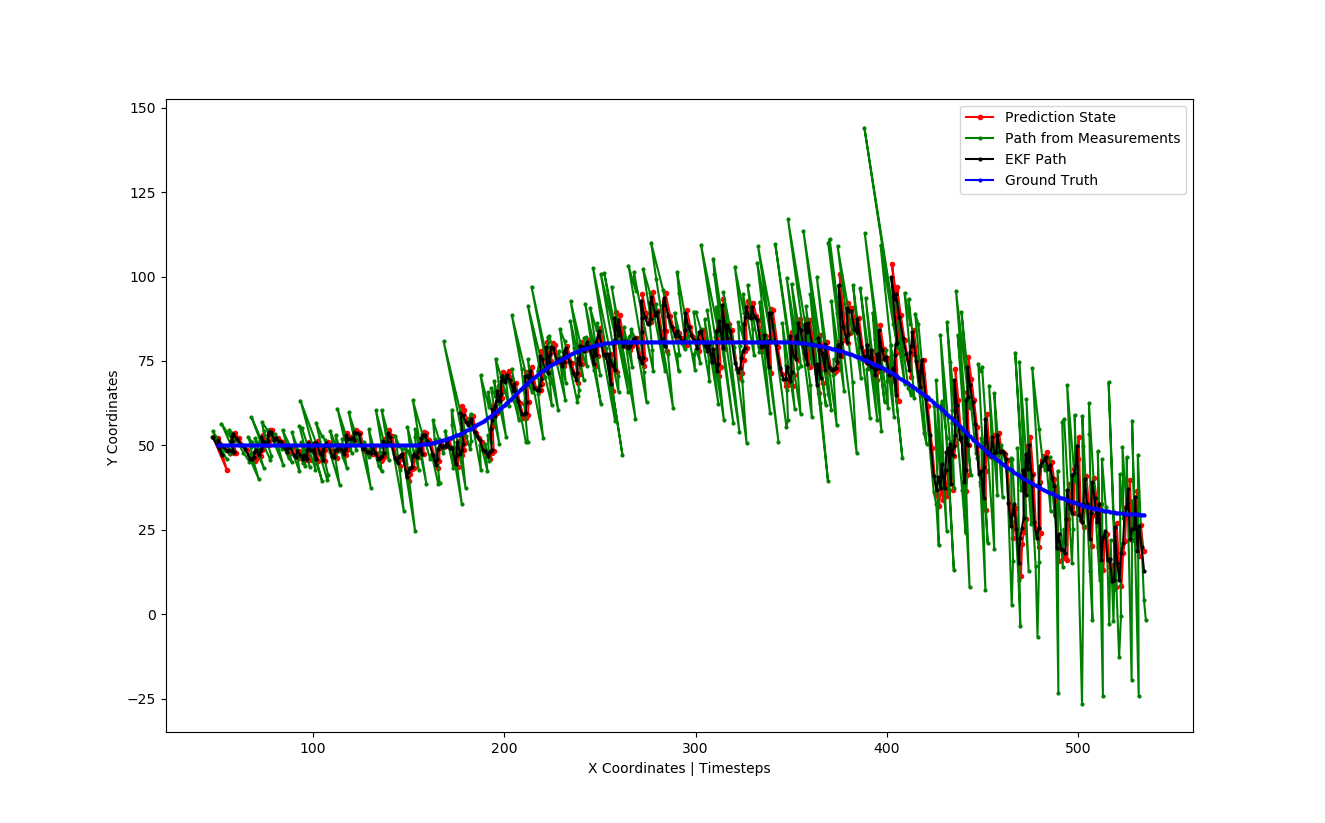
\includegraphics[width=\textwidth]{../results/path_q0_01.png}
\caption{Results: Vessel Trajectory for q value = 0.01}
\label{fig:EKF_1}
\end{figure}

\begin{figure}[]
\centering
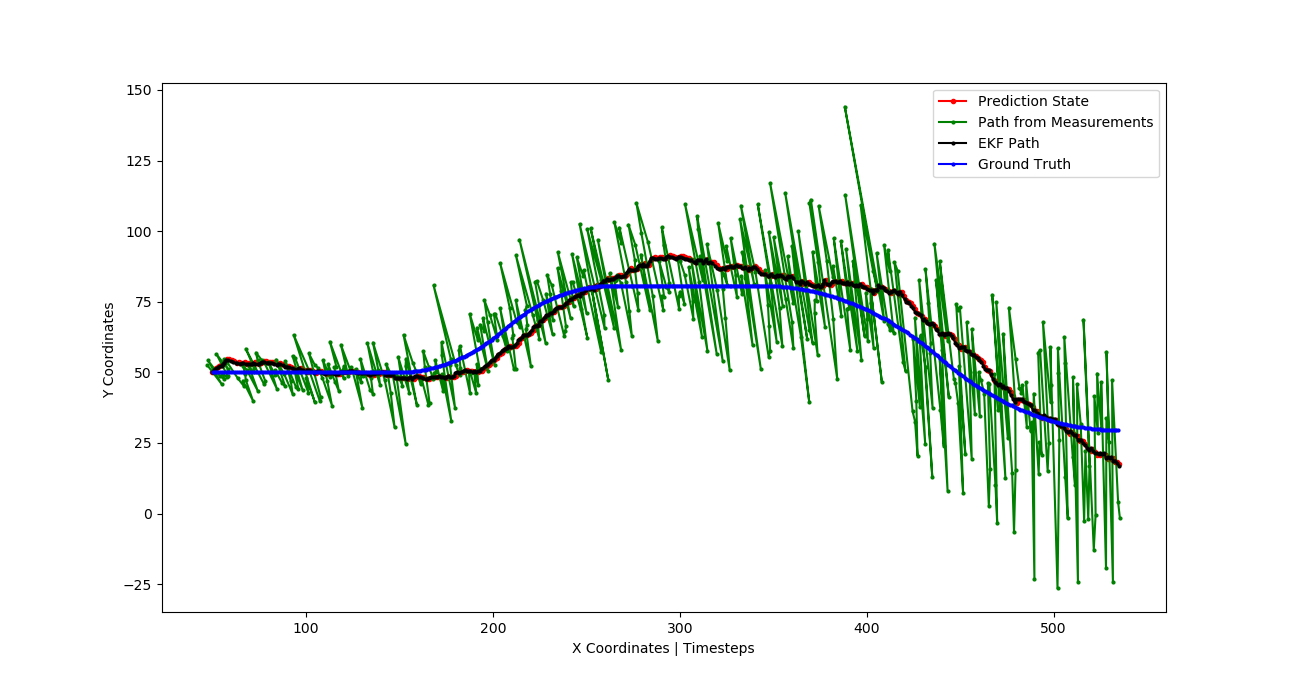
\includegraphics[width=\textwidth]{../results/path_q0_1.png}
\caption{Results: Vessel Trajectory for q value = 0.1}
\label{fig:EKF_2}
\end{figure}

\begin{figure}[]
\centering
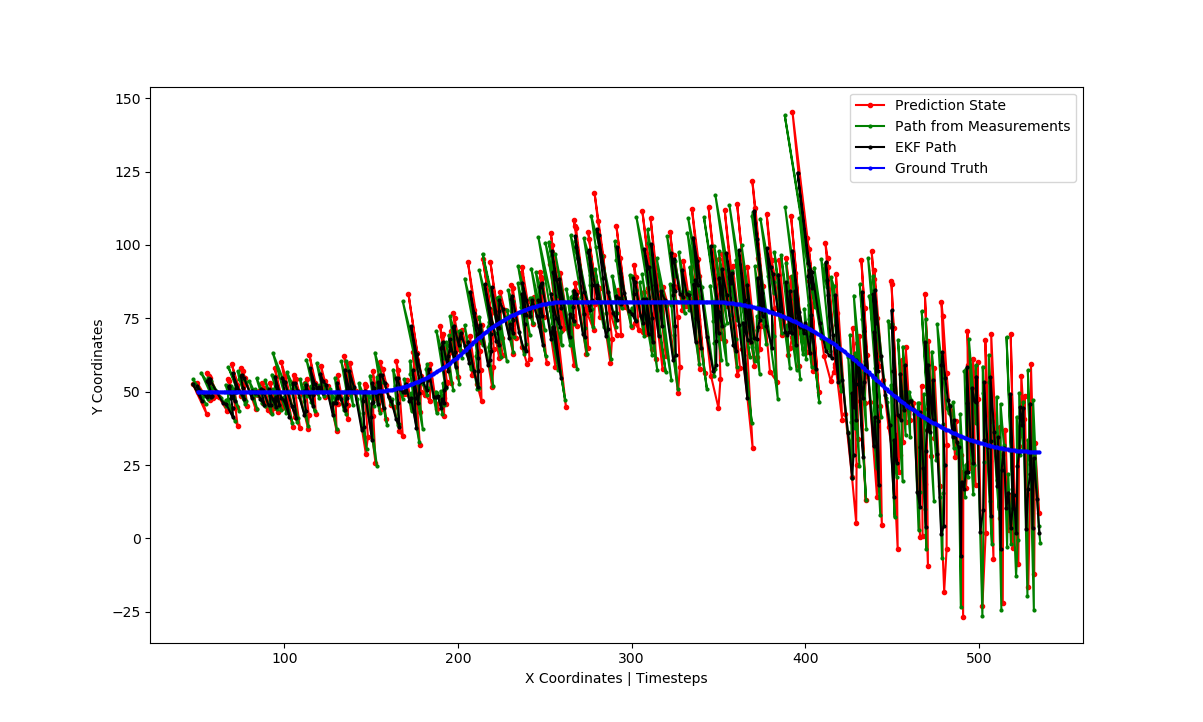
\includegraphics[width=\textwidth]{../results/path_q1.png}
\caption{Results: Vessel Trajectory for q value = 1}
\label{fig:EKF_3}
\end{figure}
  
  
  

\section{100 Monte-Carlo Samples and RMSE Error}
Run the code for three different q\_factor values and compute error statistics. Root mean squared is a metric for accuracy here. \\

$\mathrm{RMSE} = \sqrt{\frac{\sum_{t=1}^{n}{(y_t - \hat{y}_t)^2}}{n}}$\\

Where, $y_{t}$ is the ground truth data and $\hat{y}_{t}$ is the corresponding estimated data.\\

For each q scaling factor, we get RMSE values in x,y, vx and vy  for a 500 timestep sequence computed over 100 EKF samples, which are  then plotted. These plots are shown in  Fig. \ref{fig:EKF_results} for three different q scaling values. 

\begin{figure}[!th]
\centering
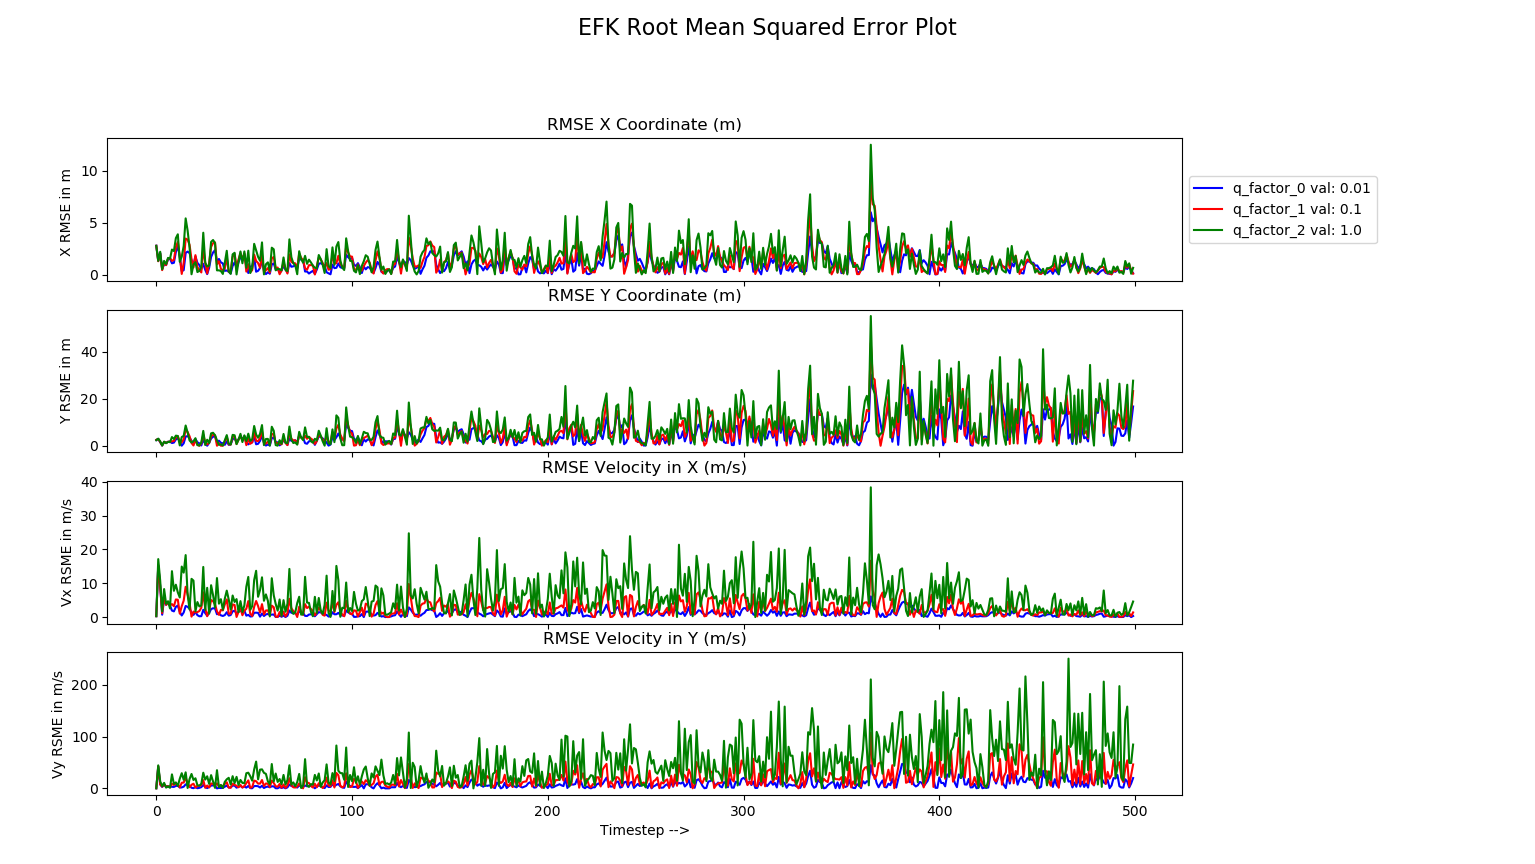
\includegraphics[width=\textwidth]{../results/EKF_results_main.png}
\caption{RMSE Errors in x,y and x,y velocities computed over 100 EKF samples.}
\label{fig:EKF_results}
\end{figure}



\section{Tuning the q factor}
Three values of q are chosen, which are passed as a list arguement to the main.py file. We can see from the Fig. \ref{fig:EKF_results}, that with increase in a scaling value, the RMSE error increases. We can thus infer that with increase in process noise, the error in performance of the EKF increases.


\section{References}
\begin{enumerate}
  \item Probabilistic Robotics, Sebastian Thrun, Wolfram Burgard, Dieter Fox.
  \item Lecture Notes on EKF, Adam Hoover,
\href{http://cecas.clemson.edu/~ahoover/ece854/lecture-notes/lecture-ekf.pdf}{\color{blue}http://cecas.clemson.edu/~ahoover/ece854/lecture-notes/lecture-ekf.pdf}  
\end{enumerate}

\end{document}



